\documentclass[11pt]{article}
\usepackage{amsmath, amssymb, amsthm}
\usepackage{graphicx}
\usepackage{hyperref}
\usepackage{geometry}
\geometry{margin=1in}

\title{Ted's Law of Karma: Covariance of Entropies and Shared Fate}
\author{Ted Strall}
\date{\today}

\begin{document}
\maketitle

\begin{abstract}
We propose a principle---\textbf{Ted's Law of Karma}---stating that 
\emph{the covariance structure of entropy streams reveals the shared fate of interdependent systems}.
By measuring entropy over time for multiple signals and computing their covariance matrix, 
the dominant eigenvalue $\lambda_1$ captures the degree of systemic alignment of uncertainty. 
We demonstrate this with a toy example and discuss implications for site reliability engineering, 
complex systems, and AI safety---including a concrete operationalization of Geoffrey Hinton's call 
for a ``maternal instinct'' in AI systems.
\end{abstract}

\section{Introduction}
Complex systems rarely fail due to one signal alone. Failures arise when uncertainties across subsystems align.
In philosophy, this interdependence is described as \emph{karma}. 
In information theory, it can be captured through entropy and covariance.

This paper introduces \textbf{Ted's Law of Karma}, unifying these perspectives into a 
measurable framework.

\section{Ted's Law of Karma}
\textbf{Statement:} \emph{The covariance structure of entropy streams reveals the shared fate of interdependent systems.}

Formally, given $n$ metric time series $\{x_i(t)\}$, define entropy streams
\[
H_i(t) = - \sum_{k} p_{i,k}(t) \log p_{i,k}(t),
\]
where $p_{i,k}(t)$ is the empirical distribution of values in a rolling window.

Construct the covariance matrix
\[
\Sigma_H(t) = \text{Cov}(H_1(t), H_2(t), \ldots, H_n(t)).
\]

Let $\lambda_1(t) \ge \lambda_2(t) \ge \cdots \ge \lambda_n(t)$ be eigenvalues of $\Sigma_H(t)$. 
A spike in $\lambda_1(t)$ indicates the emergence of a systemic mode of shared uncertainty.

\section{Toy Example}
We generate three synthetic entropy streams:
\begin{enumerate}
    \item Independent noise (baseline).
    \item Coordinated disturbance introduced at $t=50$.
\end{enumerate}

\noindent \textbf{Expected result:} Under independence, $\lambda_1$ remains small. 
When coordination occurs, $\lambda_1$ spikes. 

\begin{figure}[h]
\centering
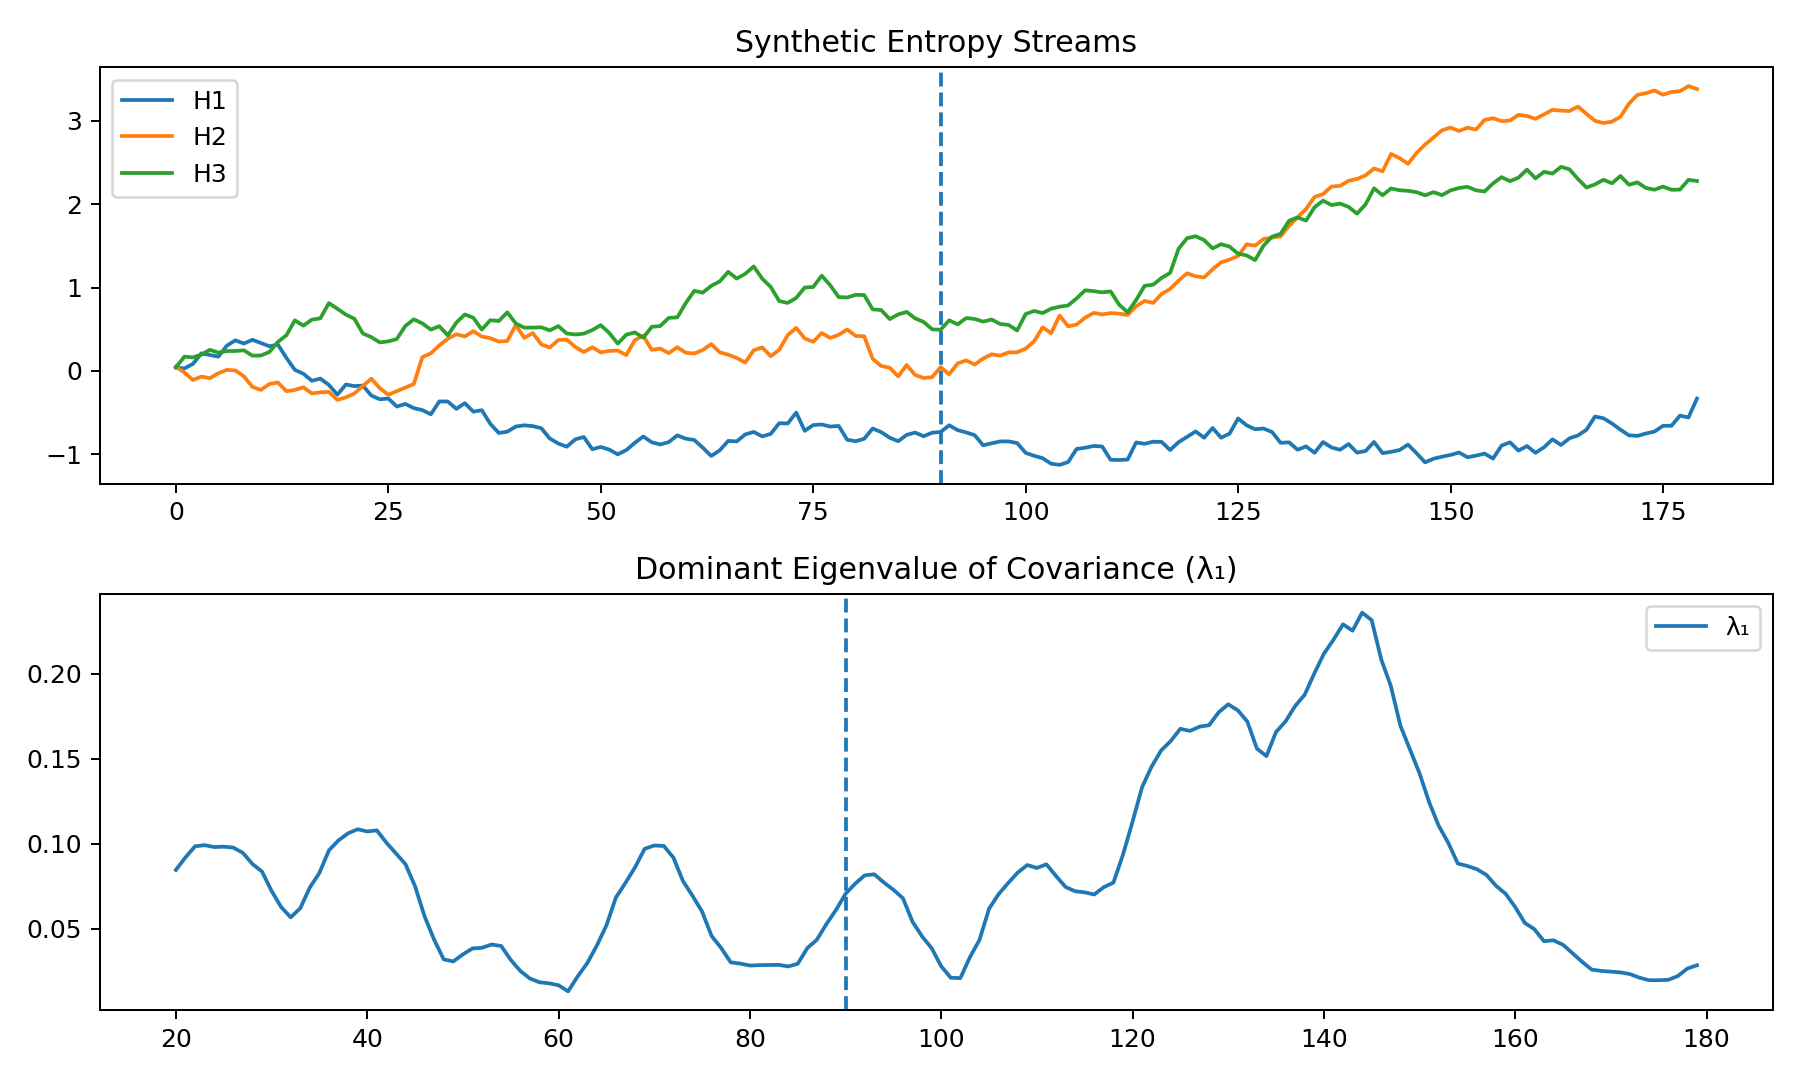
\includegraphics[width=0.8\textwidth]{toy_example_plot.png}
\caption{Toy example: entropy streams (top) and $\lambda_1$ of $\Sigma_H(t)$ (bottom). 
Spike at $t=50$ reveals systemic alignment.}
\end{figure}

\section{Implications}
\subsection{For SRE}
Eigenvalue spikes anticipate incidents by detecting alignment of uncertainties across metrics 
before threshold-based alerts fire.

\subsection{For Complex Systems}
Suggests a general mechanism for cascades: emergent failures are preceded by eigenmodes 
of entropy alignment.

\subsection{For AI Safety}
Provides a formalization of ``maternal instinct'' as sensitivity to entropy covariance. 
Systems can bias toward protective actions when shared uncertainty increases.

\section{Future Work}
\begin{itemize}
    \item Formalize within information geometry or statistical physics.
    \item Test across domains: ecosystems, economies, neuroscience.
    \item Embed entropy-covariance sensitivity in reinforcement learning agents.
\end{itemize}

\section{Conclusion}
Ted's Law of Karma compresses a universal idea: 
\emph{shared fate is visible in the covariance of entropies}.
This framing connects information theory, operations practice, and AI safety.

\appendix
\section*{Appendix A: Maxwell-Style Formulation of Ted's Law of Karma}

\paragraph{Entropy fields.}
For metric streams indexed by $i=1,\dots,n$, define rolling Shannon entropy $h_i(t)$ on a window. Stack as $\mathbf{h}(t)\in\mathbb{R}^n$. Let $\Sigma(t)=\mathrm{Cov}[\mathbf{h}(t)]$ denote the covariance of entropy streams.

\subsection*{C1. Continuity (balance) of entropy}
Each stream balances sources, damping, flux, and noise:
\begin{equation}
\dot h_i \;=\; s_i \;-\; \kappa_i h_i \;-\; \sum_{j}\nabla\!\cdot J_{ij} \;+\; \eta_i,
\end{equation}
where $s_i$ are exogenous sources, $\kappa_i\!\ge 0$ damping, $J_{ij}$ uncertainty flux from $j\!\to\! i$, and $\eta_i$ noise.

\subsection*{C2. Constitutive law (flux response)}
Linearizing around a baseline, flux follows gradients/couplings (Fick/Fourier analogue):
\begin{equation}
J_{ij} \;=\; -D_{ij}\,(h_j-h_i)
\quad\Longrightarrow\quad
\dot{\mathbf h} \;=\; -\alpha\,\mathbf h \;-\; \beta\,L\,\mathbf h \;+\; \mathbf s \;+\; \boldsymbol\eta,
\end{equation}
where $L$ is a graph Laplacian over metrics, with $\alpha,\beta\!\ge 0$.

\subsection*{C3. Correlation evolution (Lyapunov dynamics)}
Write $\dot{\mathbf h}=A\,\mathbf h+\boldsymbol\eta$ with $A=-(\alpha I+\beta L)$. Then
\begin{equation}
\dot{\Sigma}\;=\;A\Sigma + \Sigma A^\top + Q \;-\; \Gamma(\Sigma),
\label{eq:lyap}
\end{equation}
where $Q=\mathrm{Cov}[\boldsymbol\eta]$ (drive) and $\Gamma(\Sigma)$ represents control (e.g., autoscaling/rate-limits). In discrete time:
\begin{equation}
\mathbf h_{t+1} \approx A_t \mathbf h_t + \boldsymbol\varepsilon_t,\qquad
\Sigma_{t+1} \;=\; A_t \Sigma_t A_t^\top + Q_t \;-\; \Gamma_t.
\end{equation}

\subsection*{C4. Alignment law (Gauss-style)}
Define alignment density as off-diagonal mass or via the dominant eigenvalue:
\begin{equation}
\rho_{\text{align}}(t) \;=\; \sum_{i\ne j} w_{ij}\,\Sigma_{ij}(t),
\qquad
\lambda_1(t) \;=\; \lambda_{\max}\big(\Sigma(t)\big).
\end{equation}
Alignment accumulates from couplings and noise, and is drained by control:
\begin{equation}
\frac{d}{dt}\,\rho_{\text{align}} \;=\; \Phi_{\text{coupling}}(A,\Sigma) \;+\; \mathrm{tr}(WQ)\;-\;\mathrm{tr}(W\Gamma).
\end{equation}

\subsection*{Eigenmode monitor (operational early warning)}
Let $u_1(t)$ be the unit eigenvector for $\lambda_1(t)$. From \eqref{eq:lyap}:
\begin{equation}
\dot\lambda_1 \;=\; u_1^\top \dot\Sigma\, u_1 
\;\approx\; u_1^\top\!\big(A\Sigma+\Sigma A^\top + Q - \Gamma\big)u_1.
\end{equation}
If the symmetric part $\mathrm{Sym}(A)=(A{+}A^\top)/2$ loses damping (critical slowing), the $A\Sigma+\Sigma A^\top$ term becomes positive, and $\lambda_1$ rises---the measurable ``karma spike.''

\subsection*{Fitting recipe (discrete-time, practical)}
\begin{enumerate}
\item Compute $h_i(t)$: rolling Shannon entropy for each metric.
\item Fit VAR(1): $\mathbf h_{t+1}\approx A_t \mathbf h_t + \varepsilon_t$ on a sliding window.
\item Estimate $Q_t=\mathrm{Cov}[\varepsilon_t]$.
\item Propagate covariance: $\Sigma_{t+1}=A_t\Sigma_tA_t^\top+Q_t$.
\item Monitor $\lambda_1(t)$, $\mathrm{tr}(\Sigma)$, and off-diagonal mass; trigger alerts or protective bias when $\lambda_1$ spikes above baseline.
\end{enumerate}

\paragraph{Summary.}
These equations encode Ted's Law of Karma as a dynamical system: entropy streams behave like fields, their covariances evolve by Lyapunov dynamics, and eigenvalue spikes precede shared-fate events.

\begin{thebibliography}{9}
\bibitem{Shannon1948} C. Shannon. ``A Mathematical Theory of Communication.'' Bell System Technical Journal, 1948.
\bibitem{Hinton2023} G. Hinton. ``The Need for Maternal Instinct in AI.'' (Talks, 2023).
\end{thebibliography}

\end{document}
